\documentclass{article}
\usepackage[english]{babel}
\usepackage{authblk,graphicx,float}
\usepackage{amssymb}

\usepackage[letterpaper,top=2cm,bottom=2cm,left=3cm,right=3cm,marginparwidth=1.75cm]{geometry}
\usepackage{amsmath}
\usepackage{graphicx}
\usepackage[colorlinks=true, allcolors=blue]{hyperref}
\title{Project 3 Proposal  \\ \ \\IN9310 - Advanced Deep Learning for Image Analysis
}
\author{Kumar, Nikhil}

\date{\today}

\begin{document}

\maketitle

%%%%%%%%%%%%%%%%%%%%%%%%%%%%%%%%%%%%%%%%%%%%%%%%%%%%%%%%%%%%%%%%%%%%%%%%%%%%%%%%%%%%%%%%%%%%%%%%%

\section*{Project: Utilizing the Variational Bayes Autoencoder in Survival Analysis for 3D CT data}


\section{Introduction}
\subsection{Problem definition}
In medical research, particularly in survival analysis (SA), researchers face the challenge of handling complex, varied, incomplete, and censored data. Censored data occurs when the event under study (like a patient's death) hasn't occurred for various reasons—such as a patient dropping out of the study, switching hospitals, or the study ending while the patient is still alive. Traditional methods like regression analysis cannot be used effectively because they assume that the observed survival time is the actual time until the event, which is not true for censored data.   

Accurate predictions in survival analysis are vital. They allow healthcare professionals to better assess treatment effectiveness, manage disease progression, and enhance patient care. Mistakes due to misunderstood data can lead to incorrect medical guidance, affecting patient outcomes.

Historically, survival analysis has predominantly been conducted on clinical datasets, with models developed specifically for these types of data. Most benchmark datasets in this field are clinical, which has limited the diversity of models. Although there are survival analysis models that use 3D images, they typically employ simple encoder-decoder architectures without leveraging the complexities of the data. These approaches lack robustness and flexibility because they do not incorporate advanced concepts like latent variables, which are crucial for capturing deeper, more nuanced patterns in the data. 

The project introduces a novel method, the Survival Analysis Variational Autoencoder (SAVAE), that innovatively uses Variational Autoencoders (VAEs) designed for survival analysis. SAVAE addresses censored data challenges by employing a special formula and allowing for dynamic probability calculations. This method is superior to traditional survival models as it leverages latent variables for greater robustness and predictive accuracy. It has demonstrated strong and stable results across various measures on clinical datasets.

Currently, SAVAE is implemented for clinical data \cite{apellaniz2023savae}; however, there is an opportunity to extend this model to 3D image data. Such an expansion would allow the exploration of more complex medical scenarios where 3D imaging plays a critical role, such as in oncology or neurology, providing a more comprehensive tool for medical research and patient care.

By expanding SAVAE to work with both traditional clinical and 3D image data, we're not just improving how we handle censored data; we're potentially setting a new standard in the field. It also helps with other tasks like grouping similar patients, filling in missing information, and even creating realistic patient simulations for further study.


\subsection{Contributions}
The central contribution of this project is adapting the existing SAVAE model, originally developed for clinical datasets, to handle 3D image data. This adaptation involves modifying the model’s architecture to effectively process the complexities and characteristics of 3D imaging, pivotal in medical fields like radiology and oncology. Moreover, the Evidence Lower Bound (ELBO), a key component in training Variational Autoencoders, has been customized to better suit the unique demands of survival analysis with 3D imaging. By doing so, the project aims to extend the utility of survival analysis into new areas that rely heavily on detailed imaging for diagnostics and prognosis, while using established methods to handle censored data effectively within these new contexts.

\section{Related work}
\subsection{Literature}

Recent advances in medical research have shifted towards using Deep Learning (DL) to predict important health events like disease progress and patient survival. Although traditional statistical methods like the Cox proportional hazards model \cite{kraisangka2018bayesian} are commonly used, they rely on assumptions that may not hold true with complex data, such as constant hazard functions and linear relationships without interactions among variables. 

As a response, researchers have started using Deep Neural Networks (DNNs) to handle non-linear and complex relationships in data. Models like DeepSurv \cite{jared2016deep} have tried to adapt older models to capture these complexities but still assume proportional hazards. A new model, DeepHit \cite{lee2018deephit}, moves away from this assumption and has shown promising results, although it requires large datasets.

Researcher have been also focusing on imaging data. XSurv, a merging-diverging framework using PET-CT images for survival prediction in Head and Neck cancer, outperformed state-of-the-art methods in the HECKTOR 2022 challenge \cite{meng2023merging}. Another study uses a cross-modality attention-based fusion architecture to integrate modality-specific knowledge for patient survival prediction \cite{deng2024cross}.

Building on these developments, we introduce a new model called SAVAE (Survival Analysis Variational Autoencoder). SAVAE uses a flexible, generative approach with Variational Autoencoders to predict event timings more accurately and can handle different types of data, including censored data from patients who haven't yet experienced the event of interest. This makes it a versatile tool in medical research, promising better predictions and adaptability across various domains.

\section{Methods}
\subsection{Dataset}
we will be using the 197 3D CT volume along with the time and the event data \cite{simpson2024preoperative}. The publicly available data can be accessed on this website  https://www.cancerimagingarchive.net/collection/colorectal-liver-metastases. 


\subsection{VAE}
Introduced in 2013 \cite{kingma2013auto}, the Variational Autoencoder (VAE) utilizes deep neural networks for Bayesian inference on datasets where all observations \(x_i\) are independent given the latent variable \(z\). The model generates data \(x_i\) from a conditional distribution \(p_\theta(x|z)\), streamlining the Bayesian inference process. To handle the computational challenges of deriving the true posterior \(p_\theta(z|x)\), VAE employs a variational approach with a family \(q_\phi(z|x)\), optimizing parameters \(\phi\) to enhance approximation quality. To ensure the objective function is differentiable, the reparametrization trick is used. Initially, sampling directly from the encoder outputs \(\mu\) and \(\sigma\) made the process non-deterministic. To make it deterministic,  we sample from a standard normal distribution and adjust by multiplying by \(\sigma\) and adding \(\mu\), thereby enabling gradient-based optimization techniques.

\begin{figure}[H]
    \centering
    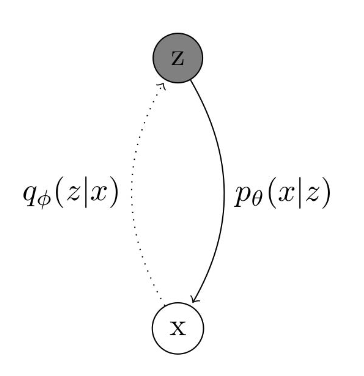
\includegraphics[width=4cm]{figures/VAE.png}
    \caption{Bayesian VAE vanilla model. The shaded circle refers to the latent variable z, and the white circle refers to the observable x. Probabilities \(p_\theta(x|z)\) and \(q_\phi(z|x)\) denote, respectively, the generative model and the variational approximation to the posterior, since the true posterior p(z|x) is unknown.}
    \label{VAE}
\end{figure}

The ELBO of the VAE is given by:

\begin{equation}
    \log p_\theta(x) \geq -D_{KL}(q_\phi(z|x) \parallel p(z)) + \mathbb{E}_{q_\phi(z|x)}[\log p_\theta(x|z)] = L(x, \theta, \phi),
\end{equation}

Instead of directly maximizing \(\log p_\theta(x)\), we focus on maximizing the lower bound on the right-hand side of Equation 1, which includes the Kullback-Leibler divergence and the log likelihood.

\subsection{Survival Analysis}
In survival analysis \cite{clark2003survival}, we consider \(N\) observations each represented by triplets \(D = (x_i, t_i, d_i)\). Each \(x_i\) is an L-dimensional vector representing image data, \(t_i\) is the time-to-event, and \(d_i\) is a censor indicator where 0 denotes censored data and 1 denotes an observed event. SA models employ these image data vectors to define the probability density function \(p(t|x)\), the hazard rate \(h(t|x)\), and the survival function \(S(t|x) = 1 - F(t|x)\), where \(F(t|x)\) is the cumulative distribution function. These functions collectively form the foundation for modeling time-to-event data.

\begin{equation}
p(t|x) = h(t|x)S(t|x).
\end{equation}

\subsection{SAVAE-ELBO}
In our approach, we use a VAE (Variational Autoencoder) architecture to expand on the ELBO (Evidence Lower Bound) concept from standard VAE models. Our model, SAVAE, operates under the assumption that the two data-generating models,  \( p_{\theta_1} (x|z) \) and \( p_{\theta_2} (t|z) \),  are independent when \( z \) is known. This independence means that with knowledge of \( z \), we can generate either \( x \) or \( t \) separately. We do not allow \( Z \) to learn from \( t \) because \( t \) is not always available for all patients due to censorship. Furthermore, the VAE setup implies that each element within the data vector \( x \) is also independent from the others, provided \( z \) is given.

\begin{equation}
    p(x, t, z) = p_{\theta_1}(x \mid z) p_{\theta_2}(t \mid z) p(z) = p_{\theta}(x, t \mid z) p(z) 
\end{equation}

\begin{figure}[H]
    \centering
    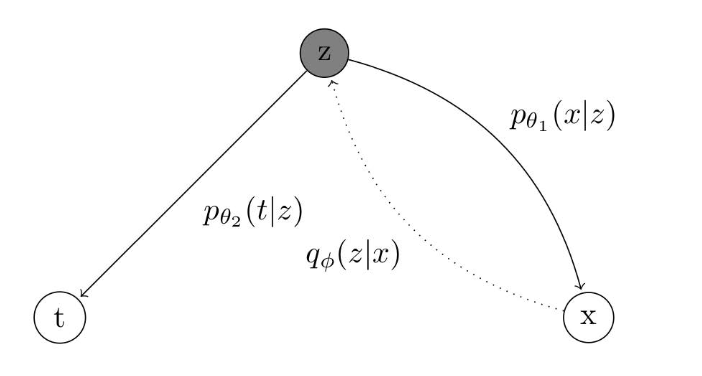
\includegraphics[width=8cm]{figures/SAVAE.png}
    \caption{The SAVAE Bayesian model is depicted with a graphical representation where the shadowed circle represents the latent variable, and the white circles denote the observables. In this model, the probabilities \(p_{\theta_1}(x|z)\) and \(p_{\theta_2}(t|z)\) represent the generative models, while \(q_\phi(z|x)\) is the variational approximation to the posterior. This approximation is necessary because the true posterior \(p(z|x)\) is unknown.
}
    \label{SAVAE}
\end{figure}

The model assumes that we know the distribution types of \( p_{\theta_1} (x \mid z) \) and \( p_{\theta_2} (t \mid z) \), but not the specific parameters \( \theta_1 \) and \( \theta_2 \). Given these assumptions, 
We compute the ELBO (Evidence Lower Bound) in a manner similar to the standard VAE. First, the conditional likelihood of a set of points \(\{x_i, t_i\}_{i=1}^N\) can be expressed as follows:


\[
\log p_{\theta}(x_1, x_2, \ldots, x_N , t_1, t_2, \ldots, t_N \mid z) = \sum_{i=1}^N \log p_{\theta}(x_i, t_i \mid z)
\]

\begin{equation}
= \sum_{i=1}^N \left(\log p_{\theta_2}(t_i \mid z) + \sum_{l=1}^L \log p_{\theta_1}(x_i^l \mid z)\right) 
\end{equation}

where the expected conditional likelihood can be expressed as:

\[
E_z \left[ p_\theta (x, t \mid z) \right] = \int p_\theta (x, t \mid z) p(z) \, dz = \int \frac{p_\theta(x,t,z)}{p(z)} p(z) \, dz
\]
\begin{equation}
=\int p_\theta(x,t,z) \, dz = p_\theta(x,t) = \int p_\theta(x,t,z) \cdot \frac{q_\phi(z|x)}{q_\phi(z|x)} \, dz 
\end{equation}
\[
= \mathbb{E}_{q_\phi(z|x)} \left[ \frac{p_\theta(x,t,z)}{q_\phi(z|x)} \right]
\]

As the interest lies in computing the log-likelihood:
\begin{equation}
\log p_\theta(x, t) = \log \left[ \mathbb{E}_{q_\phi(z|x)} \left[ \frac{p_\theta(x,t,z)}{q_\phi(z|x)} \right] \right]
\end{equation}
\[
 \geq \mathbb{E}_{q_\phi(z|x)} \left[ \log \left( \frac{p_\theta(x,t,z)}{q_\phi(z|x)} \right) \right],
\]
where the inequality comes from applying Jensen’s inequality.
The modeling choice for \( p_\theta(x, t, z) \) is defined as \( p_{\theta_1}(x|z) p_{\theta_2}(t|z) p(z) \), following the structure of a directed graphical model. This approach simplifies the joint probability distribution by leveraging conditional probabilities and assumed independences. Then, this could be rearranged as:

\[
\mathbb{E}_{q_\phi(z|x)} \left[ \log \left( \frac{p_\theta(x, t, z)}{q_\phi(z|x)} \right) \right] = \int q_\phi(z|x) \log \left( \frac{p_{\theta_1}(x|z) p_{\theta_2}(t|z) p(z)}{q_\phi(z|x)} \right) dz
\]

\[
= -\int q_\phi(z|x) \log \left( \frac{q_\phi(z|x)}{p(z)} \right) dz + \int q_\phi(z|x) \left[ \log p_{\theta_1}(x|z) + \log p_{\theta_2}(t|z) \right] dz
\]
\begin{equation}
= -D_{\text{KL}}(q_\phi(z|x) \parallel p(z)) + \mathbb{E}_{q_\phi(z|x)} \left[ \log p_{\theta_1}(x|z) + \log p_{\theta_2}(t|z) \right]
\end{equation}
\[
= L(x, \theta_1, \theta_2, \phi)
\]
After computing this ELBO, it can be seen that it is similar to the Vanilla VAE’s one (Equation 1). The only difference lies in the reconstruction term, which is expressed differently in order to explicitly distinguish between the covariates and the time-to-event.
\[
L(x, \theta_1, \theta_2, \phi)=
\]
\begin{equation}
\frac{1}{N} \sum_{i=1}^N \left( -D_{KL}(q_\phi(z|x_i) \parallel p(z)) + \log p_{\theta_2}(t_i|g_\phi(x_i, \epsilon_i)) + \sum_{l=1}^L \log p_{\theta_1}(x_{li}|g_\phi(x_i, \epsilon_i)) \right).
\end{equation}
In terms of implementation, three DNNs have been used. Note that the decoder DNNs output the parameters of each distribution.

\subsubsection{Divergence computation}

SAVAE assumes that \( q_\phi(z|x) \) follows a multidimensional Gaussian distribution, characterized by a vector of means \( \mu \), with each element denoted as \( \mu_j \), and by a diagonal covariance matrix \( C \). The main diagonal of \( C \) comprises the variances \( \sigma_j^2 \). This can be stated as:

\begin{equation}
-D_{KL}(q_\phi(z|x) \parallel p(z)) = \frac{1}{2} \sum_{j=1}^J \left(1 + \log(\sigma_j^2) - \mu_j^2 - \sigma_j^2\right),
\end{equation}

where \(J\) is the dimension of the latent space \(z\). This means that the Kullback-Leibler divergence from the ELBO, referred to as Equation 8 can be calculated analytically.

\subsubsection{Time modelling}
Handling survival data is challenged by censorship, where true survival times remain unknown, leading to incomplete observations. The SAVAE model addresses this by incorporating both censored (\(d_i=0\)) and uncensored (\(d_i=1\)) data to enhance parameter estimation accuracy. This integration is captured through the model's time probability density function (pdf), expressed as:

\begin{equation}
p_{\theta_2} (t_i|g_\phi(x_i, \epsilon_i)) = h(t_i|g_\phi(x_i, \epsilon_i))^{d_i} S(t_i|g_\phi(x_i, \epsilon_i)).
\end{equation}

This equation adapts the hazard and survival functions based on the censorship indicator \(d_i\), improving the model's reliability across different data scenarios.

The SAVAE model primarily employs the Weibull distribution for time-to-event data, which supports varying hazard functions and allows flexibility in the choice of distribution. The Weibull distribution is defined as follows:

\begin{equation}
p(t; \alpha, \lambda) = \frac{\alpha}{\lambda} \left(\frac{t}{\lambda}\right)^{\alpha-1} \exp\left(-\left(\frac{t}{\lambda}\right)^\alpha\right),
\end{equation}
\begin{equation}
S(t; \alpha, \lambda) = \exp\left(-\left(\frac{t}{\lambda}\right)^\alpha\right),
\end{equation}
\begin{equation}
h(t; \alpha, \lambda) = \frac{\alpha}{\lambda} \left(\frac{t}{\lambda}\right)^{\alpha-1}.
\end{equation}

These equations provide the basis for integrating different distributions, such as the exponential distribution (a special case of the Weibull with \(\alpha = 1\)), into the SAVAE model, demonstrating its versatility and capacity to predict the distribution parameters for each patient and calculate various statistics like means, medians, and percentiles.

\subsubsection{Marginal log-likelihood computation}
In the SAVAE model, Gaussian distributions are used for real-numbered variables due to their symmetry and continuous nature for 3D images.

\subsection{Training Details}
The SAVAE model would be implemented using PyTorch and involves three DNNs: one encoder and two decoders, focusing on images and time parameters. The encoder features a simple Gaussian structure with a 3D Convolution layers similar to U-Net model, outputting to a fixed five-dimensional or 10-dimensional latent space. This space feeds into two decoders, with 3D Transpose convolution layer for image decoder and linear layers for time decoder. Training span 300 epochs with batch sizes of 64, including an Early Stop mechanism for efficiency.


\begin{figure}[H]
    \centering
    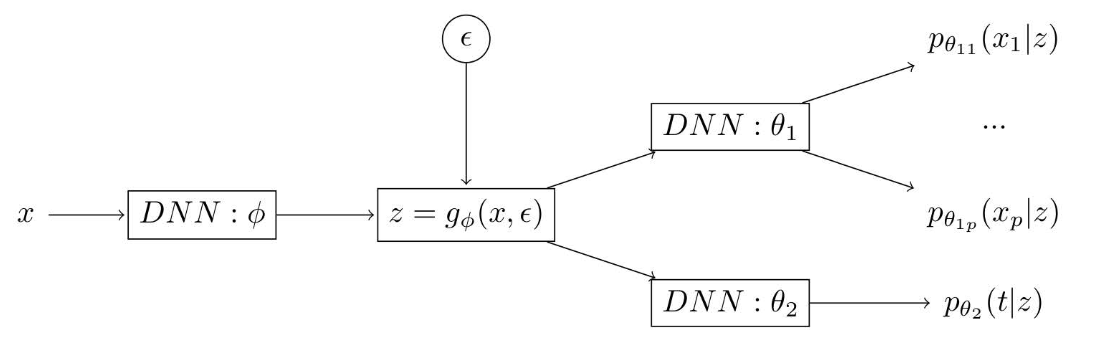
\includegraphics[width=13cm]{figures/DNN.png}
    \caption{SAVAE implementation using DNNs. One of them acts as an encoder which has the covariates vector as input. The other two act as decoders, one for the covariates and the other one for the time. }
    \label{DNN}

\end{figure}
\subsection{Evaluation metrics}
In Survival Analysis, datasets are comprised of \(N\) triplets \(D = (x_i, t_i, d_i)\), where \(x_i\) is an \(L\)-dimensional vector of covariates, \(t_i\) represents the time to event, and \(d_i\) serves as the censoring indicator. The primary evaluation metric, the C-index, gauges the correlation between predicted risks and observed event times, and is adapted for time-varying risks through the time-dependent C-index:


\begin{equation}
C_{\text{index}} = P(\hat{F}(t|x_i) > \hat{F}(t|x_j) | d_i = 1, t_i < t_j, t_i \leq t),
\end{equation}

Further, the Brier Score (BS) quantifies prediction errors, adjusted for censored data using Inverse Probability of Censoring Weighting (IPCW), which assesses both calibration and discrimination capabilities of models. The Integrated Brier Score (IBS) aggregates this assessment over all possible times, providing a comprehensive measure of model performance:


\begin{equation}
IBS(t_{\text{max}}) = \int_0^{t_{\text{max}}} BS(t) \, dt.
\end{equation}

These metrics collectively enhance the robust evaluation of SA models, incorporating accuracy, calibration, and adaptability to temporal changes in risk.

\section{Results}
\subsection{Experimental results}

Employing Variational Autoencoders, SAVAE enhances accuracy by leveraging latent variables to uncover complex data patterns. Tested on clinical datasets, the model demonstrated robustness and superior predictive capabilities. Preliminary results also suggest potential applicability to 3D image data, promising broader utility in medical research. The belief is to achieve a better C-index and IBS scores compare to the other models. Overall, SAVAE represents a significant advancement in the predictive modeling of patient outcomes.

\subsection{Experimental discussion}
SAVAE may achieve improved predictive accuracy and robustness compared to traditional models, highlighting its capacity to uncover complex data patterns missed by previous methodologies.  These results not only align with but also extend current literature by offering a flexible, more accurate model for diverse medical datasets. Overall, SAVAE's innovative approach sets a new benchmark in predictive modeling.



\bibliographystyle{plain}  
\bibliography{bibl.bib}
\cleardoublepage





\end{document}